\documentclass{article}

\usepackage{neurips_2026}

\usepackage[utf8]{inputenc}
\usepackage[T1]{fontenc}
\usepackage{hyperref}
\usepackage{url}
\usepackage{booktabs}
\usepackage{amsfonts,amsmath,amssymb,amsthm}
\usepackage{nicefrac}
\usepackage{microtype}
\usepackage{xcolor}
\usepackage{graphicx}
\usepackage{caption}
\graphicspath{{../figures/}}

\newtheorem{proposition}{Proposition}
\newcommand{\dprime}{$d'$}
% Total GPU-hours: Misha H100 13.2 (scripts/compute_hours.sh) + Modal B200 13.0, H100 12.2, L40S 13.0 (usage dashboard,
% Oct 2026, dollars / list rate). Used in Appendix B and the checklist.
\newcommand{\gpuhours}{51}

\title{Transformers Find the Item but Misread It:\\Locating versus Readout in Working Memory}

\author{%
  Anonymous Author(s) \\
  Affiliation \\
  Address \\
  \texttt{email} \\
}

\begin{document}

\maketitle

\begin{abstract}
Large language models fail the N-back task in a human-like way: accuracy falls steeply as N grows, and most errors are false alarms on near-target lures. A prominent account attributes this limit to the precision of softmax attention, which must single out one past position among many. We test that account directly in 15 pretrained models (Pythia 70M--6.9B, GPT-2 124M--1.5B, Qwen2.5 0.5B--14B) and in minimal transformers trained from scratch. We separate each error into a \emph{locating} failure (attention lands on the wrong item) and a \emph{readout} failure (attention lands on the right item but the answer is still wrong). Three results favour readout. First, the heads that carry the task attend to the target on about 90\% of misses. Second, linear probes on the residual stream separate true matches from lures almost perfectly (median AUC 0.98--1.00) while the model's own answer barely does (0.58--0.63), including on the model's own false alarms. Third, sharpening the identified heads barely changes performance (median $\Delta d'=+0.05$), whereas removing the letter identity of non-target items raises it in 42 of 43 model$\times$N cells (median $+0.60$, up to $+1.78$ in Qwen2.5-14B), five times the gain of a recent content-suppression intervention we replicate. In minimal models, softmax precision does limit a one-layer, residual-free transformer, but depth and a residual stream remove the limit entirely, and even there accuracy tracks how content is used rather than how sharply position is coded. Working-memory limits in transformers are therefore limits of readout under interference, not of attention precision.
\end{abstract}

\section{Introduction}
\label{sec:intro}

Working memory, the ability to hold and use a few items over seconds, has a famously small capacity in humans \citep{cowan2001magical,ma2014changing}. The N-back task probes it directly: for each item in a stream, say whether it matches the one N steps back \citep{kirchner1958age}. People get worse as N grows, and their errors concentrate on lures, items that match at N$\pm$1 \citep{kane2007nback}. Executive-attention accounts explain this as a failure to select the target against competitors \citep{engle2002executive}.

Pretrained language models show the same signature even though the whole sequence sits in their context \citep{gong2024chatgpt,hu2025nback}. Because nothing has been forgotten, the bottleneck must lie in \emph{retrieval}. Two mechanistic accounts compete. The \emph{precision} account holds that softmax attention cannot concentrate enough mass on position $i-N$ when many keys compete, so nearby items leak in \citep{gong2024selfattention,velickovic2025softmax}. The \emph{interference} account holds that the model can find the target, but the content of other items is entangled with it in the residual stream and corrupts the decision \citep{xiong2026superposition}. The two predict different things: if attention is imprecise, errors should come with attention in the wrong place and sharpening attention should help; if readout is the bottleneck, errors should occur with attention in place, the needed information should be present in the representation, and removing competing content should help.

We test both predictions with a common set of stimuli, thresholds and interventions across 15 pretrained models and a family of minimal transformers. Our contributions:
\begin{itemize}
  \item \textbf{A locating-versus-readout decomposition} (Section~\ref{sec:locate}). Content-addressed heads place attention on the target line on about 90\% of misses; lure false alarms come from heads landing on the same-letter lure. Probes show that whether a match sits at $i-N$ or at a lure offset is linearly decodable in the residual stream, and remains so on the model's own false alarms.
  \item \textbf{A causal contrast on one axis} (Section~\ref{sec:causal}, Fig.~\ref{fig:causal}). Ablating the identified heads costs a median 0.93 \dprime{}; sharpening them gains a median 0.05; removing distractor content gains 0.60, with sequence-level bootstrap intervals for every cell.
  \item \textbf{Where precision binds} (Section~\ref{sec:theory}). We show when the softmax precision bound constrains capacity (one layer, no residual stream) and why depth removes it, and find that even there accuracy tracks the use of content, not the sharpness of position.
  \item \textbf{Architecture and development} (Section~\ref{sec:arch}). Fixed-state recurrent models with enough state solve the task, while a selective state-space model declines with N like attention; N-back heads appear early in Pythia training.
\end{itemize}

\begin{figure}[t]
  \centering
  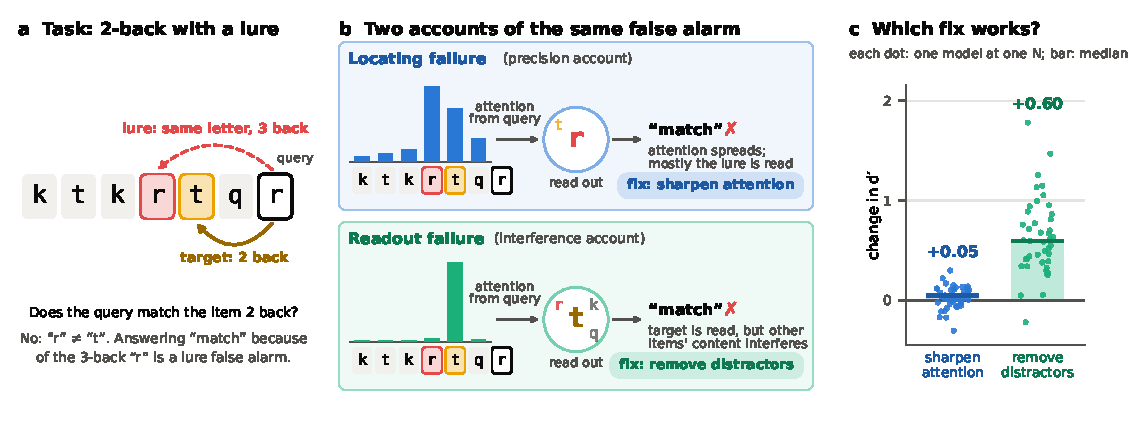
\includegraphics[width=\textwidth]{fig1_overview.pdf}
  \caption{\textbf{Overview.} (a) N-back with a lure: the target is the item N back; a lure repeats the query letter at N$\pm$1. (b) Two accounts of an error. (c) Across 15 LLMs and N = 2--4, sharpening the heads that carry the task barely changes \dprime{}, while removing the letter identity of non-target items raises it substantially (medians; Section~\ref{sec:causal}).}
  \label{fig:overview}
\end{figure}

\section{Related work}
\label{sec:related}

\textbf{Working memory in LLMs.} \citet{gong2024chatgpt} measured N-back capacity in ChatGPT and found human-like declines; \citet{gong2024selfattention} trained small transformers on N-back and related the decline to attention entropy. \citet{hu2025nback} showed that weaker models drift to an easier task, a confound we control by reporting the best-fitting $k$ for every cell. \citet{zhang2024wmreasoning} relate working-memory tests to reasoning limits. Closest to us, \citet{xiong2026superposition} show that LLMs fail working-memory tasks that a two-layer transformer solves, attribute the failure to interference among entangled item representations, and report gains from suppressing letter-identity directions, selected as the best configuration of a sweep on the evaluation trials. We replicate their intervention with held-out selection and compare it directly with head sharpening and with targeted distractor suppression.

\textbf{Softmax precision.} Softmax attention disperses as the number of keys grows \citep{velickovic2025softmax,hayase2026critical}; scalable softmax \citep{nakanishi2025scalable} and sigmoid attention \citep{ramapuram2024sigmoid} change this behaviour. Expressivity results bound what one attention layer can compute \citep{hahn2020limitations,sanford2023representational}. We use these ideas to state the N-back-specific bound and test whether it is the binding constraint.

\textbf{Mechanistic interpretability.} We build on circuit analyses \citep{elhage2021framework,wang2023ioi}, induction heads \citep{olsson2022induction}, retrieval heads \citep{wu2024retrieval}, and activation and attribution patching \citep{zhang2024patching,kramar2024atp}. Recurrent and state-space baselines follow \citet{hochreiter1997lstm,orvieto2023lru,gu2023mamba,katharopoulos2020linear}; associative recall in such models is studied by \citet{arora2023zoology,jelassi2024repeat}.

\section{Setup}
\label{sec:setup}

\textbf{Task and stimuli.} Sequences of 24 letters from a 20-consonant alphabet, with match rate fixed per N and four planted lures per test sequence (a letter repeating the query at N$\pm$1 or another non-target offset, never creating a match). LLM prompts show three solved demonstration sequences, then the test sequence one item per line (``\texttt{k -}'', ``\texttt{t m}''), with correct answers shown for earlier items (\emph{feedback} condition). The score at item $i$ is $\log p(\texttt{m}) - \log p(\texttt{-})$ at the letter token. Thresholds are calibrated on 200 held-out sequences per model, N and condition; all metrics use 1,000 test sequences. A chat format following \citet{gong2024chatgpt} is used for Qwen2.5-Instruct models (Appendix~\ref{app:methods}).

\textbf{Measures.} Sensitivity \dprime{} with the log-linear correction \citep{hautus1995corrections}, hit and false-alarm (FA) rates, FA rates split by lure offset, and the best-fitting $k$ (the $k$-back rule the model's answers fit best) to detect task drift.

\textbf{Models.} Pythia 70M--6.9B \citep{biderman2023pythia}, GPT-2 124M--1.5B \citep{radford2019gpt2} and Qwen2.5 0.5B--14B \citep{qwen2025qwen25}. Minimal models are attention-only transformers trained from scratch to convergence, varied in depth, residual stream, position encoding and attention normalization (Appendix~\ref{app:methods}).

\textbf{Heads.} For each model and N we rank heads by activation patching from a clean to a corrupted run in which the correct answer flips, scoring the fraction of the mean clean--corrupt logit gap that patching one head recovers \citep{zhang2024patching}. One head typically dominates and is shared across N; at N = 2 the top head recovers 16--73\% of the gap.

\section{Behaviour: the decline and its lures}
\label{sec:behaviour}

All 15 models decline steeply with N (Fig.~\ref{fig:behaviour}a--c; Table~\ref{tab:l2}). Median \dprime{} falls from 2.57 at N = 1 (range 1.25--4.28) to 0.91 at N = 4 and 0.52 at N = 6. Scale helps at N = 1 but little beyond: Qwen2.5-14B reaches 4.28 at N = 1 and 1.15 at N = 6. Errors are dominated by lures (Fig.~\ref{fig:behaviour}d): at N = 2 the median FA rate is 0.79 on lures at N$\pm$1 against 0.04 on non-lure items. Task drift appears only at large N in small models (best-fitting $k<N$ in 14 of 90 base-model cells, all at N$\ge$4). The chat format reproduces the decline in Qwen2.5-Instruct 0.5B--7B (\dprime{} from 1.8--2.0 at N = 1 to 0.4--0.7 at N = 6; Appendix~\ref{app:results}).

\begin{figure}[t]
  \centering
  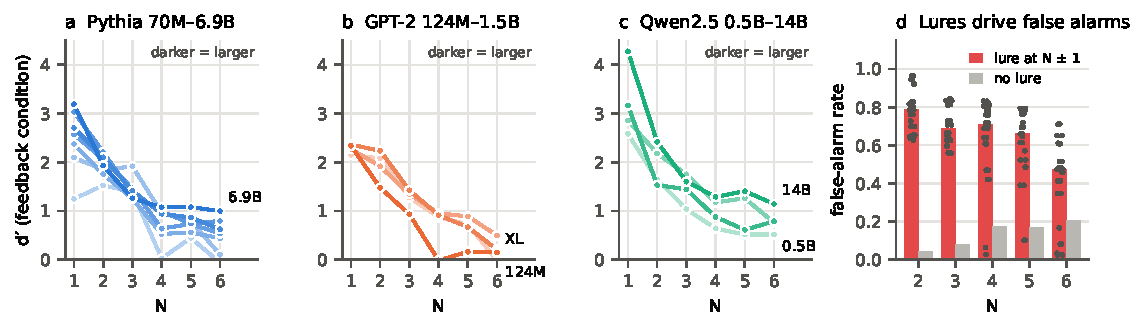
\includegraphics[width=\textwidth]{fig3_llm_behaviour.pdf}
  \caption{\textbf{Behaviour.} (a--c) \dprime{} versus N for three model families; darker lines are larger models. (d) False-alarm rates on lures at N$\pm$1 (red; dots are models) and on non-lure items (gray), medians over 15 models.}
  \label{fig:behaviour}
\end{figure}

\section{When does attention precision bind?}
\label{sec:theory}

Consider the minimal model of \citet{gong2024selfattention}: one attention layer, no residual stream and no MLP, with output $o_i=\sum_j a_{ij}v_j$, a linear decision on $o_i$, and logits $s_{ij}=c(x_i,x_j)+p(i-j)$ (a content and a position term).

\begin{proposition}[the readout is a mass test]\label{prop:mass}
In this model the decision is linear in $\sum_j a_{ij} v_j$, and no linear function of a convex combination of letter embeddings can test whether two letters are equal. The match signal must therefore be carried by how the attention distribution differs between match and non-match trials.
\end{proposition}

\begin{proposition}[softmax dispersion]\label{prop:dispersion}
If $K$ keys have logits at least $\Delta$ below the target's, the target receives mass at least $1/(1+Ke^{-\Delta})$; keeping it above $1-\epsilon$ requires $\Delta\ge\log(K/\epsilon)$. A lure shares the target's content, so only the position term separates them, and the lure-to-target mass ratio is $e^{-\delta_P}$ with $\delta_P=p(N)-p(N\pm1)$.
\end{proposition}

\begin{proposition}[depth removes the bound]\label{prop:depth}
With two layers, a residual stream and an absolute or rotary position code, a first-layer head can copy $x_{i-N}$ into position $i$ with margin growing in the weight norm, and the equality test can then be computed in the residual stream, outside the softmax. A monotone recency bias (ALiBi, or no position code) cannot single out offset $N$ in one head.
\end{proposition}

Proofs are in Appendix~\ref{app:theory}. Figure~\ref{fig:minimal} tests the propositions. The one-layer model declines with N (\dprime{} 2.67 to 2.15 over 50 seeds; panel a). Unnormalized sigmoid attention and top-$k$ attention raise and flatten the curve, while scalable softmax does not (panel b), as Proposition~\ref{prop:dispersion} predicts for a normalization-driven limit. With two layers and a residual stream the decline disappears: \dprime{} is 6.4--7.2 at every N with learned positions, 5.4--5.8 with sinusoidal and 4.5--5.9 with rotary codes, and 7.7--7.8 for a single model trained on all N with a cue (panel c); ALiBi and no-position models fail at every N (\dprime{} 1.3--1.8), as Proposition~\ref{prop:depth} predicts.

Is dispersion the binding constraint even in the one-layer model? Decomposing the logits of 720 trained checkpoints, the position margin $\delta_P$ does not shrink as N grows (4.5 at N = 1, 6.7 at N = 5). Across the 300 checkpoints of the main configuration, $\delta_P$ predicts neither lure false alarms (Spearman $\rho=-0.03$) nor \dprime{} ($\rho=-0.05$; Fig.~\ref{fig:minimal}d). What does predict \dprime{} is the size of the difference in target attention between match and non-match trials ($\rho=0.62$; leave-one-N-out $R^2=0.37$; panel e), as Proposition~\ref{prop:mass} implies. The sign of that difference changes with N: every seed attends more to the target on match trials at N = 1, but only 48\% do at N = 4 and 18\% at N = 6 (panel f); the rest attend away from a matching letter. Consistent with Proposition~\ref{prop:mass}, every post-hoc edit of the attention pattern (an oracle on $i-N$, or removing off-target mass) lowers \dprime{}, because off-target mass is part of the code (Appendix~\ref{app:results}). Precision bounds the minimal model, but the decline is shaped by how content is read out.

\begin{figure}[t]
  \centering
  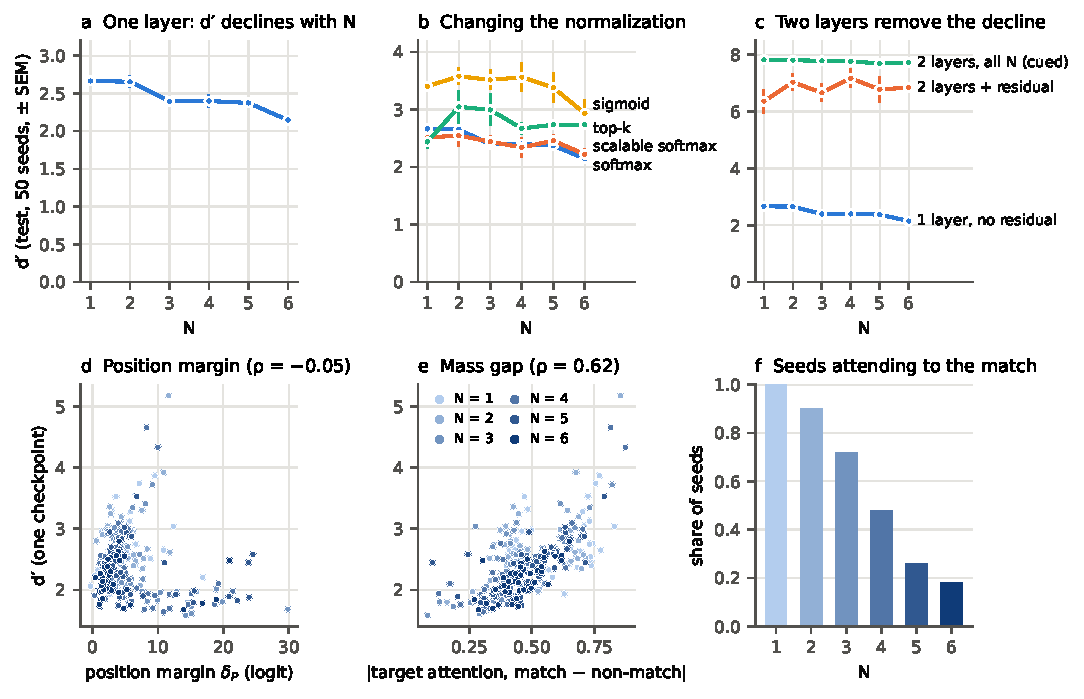
\includegraphics[width=\textwidth]{fig2_minimal_models.pdf}
  \caption{\textbf{Minimal models.} (a) The one-layer, residual-free model declines with N at convergence (50 seeds, $\pm$SEM). (b) Sigmoid and top-$k$ attention flatten the decline; scalable softmax does not. (c) Two layers with a residual stream remove it, for one N per model or all N in one cued model. (d, e) Across 300 one-layer checkpoints (50 seeds $\times$ N = 1--6; darker = larger N), \dprime{} is unrelated to the position margin $\delta_P$ but tracks the absolute difference in target attention between match and non-match trials. (f) Share of seeds whose target attention is higher on match trials.}
  \label{fig:minimal}
\end{figure}

\section{Locating versus readout in LLMs}
\label{sec:locate}

\textbf{Do errors come with attention in the wrong place?} For every test item we measure the attention of the top-5 heads from the query letter to the whole line (letter, answer, newline) of item $i-N$ and of its neighbours $i-N\pm1$, and call the item \emph{located} when the target line receives at least as much attention as either neighbour. On correct matches the heads locate the target in a median 88--91\% of items; on correct non-matches only about 25\%, because nothing at $i-N$ matches: the heads are content-addressed. On misses the target is located just as often: attention is elsewhere on only 16\%, 7\% and 8\% of misses at N = 2, 3 and 4 (Fig.~\ref{fig:locate}a; medians over 14 models, excluding GPT-2 Large, whose top heads attend to none of the three lines). A logistic probe trained on correct trials then reads the answer from the heads' concatenated outputs: the heads' output already pointed to the wrong answer in 41--57\% of misses, and to the right answer, lost in later layers, in 27--43\%. Lure false alarms are the mirror image: on 91--96\% of them the target line loses to a neighbouring line, typically the lure's, which holds the matching letter.

\textbf{Is the position of the match represented?} Matches and lures both contain the query letter, so only its position separates them. A logistic probe (5-fold, split by sequence) reads match versus lure from the query token's residual stream at nine depths (Fig.~\ref{fig:locate}b,c). The model's own score separates them with median AUC 0.63 (N = 2) and 0.58 (N = 3). The probe reaches a median of 1.00 and 0.98 at the best depth; the input embedding is at chance. On the model's own lure false alarms, the probe still calls a median 95\% (N = 2) and 86\% (N = 3) of items lures. The largest model shows the same gap: in Qwen2.5-14B the model's own score separates matches from lures with AUC 0.81 and 0.64, the probe with 1.00 and 0.997, and the probe calls 99.8\% and 95\% of the model's lure false alarms lures. The information peaks in middle layers and declines toward the output (N = 3: 0.92 at the last layer), and the top heads' outputs carry less of it (AUC 0.71--1.00) than the residual stream. Only in the GPT-2 family at N = 3 is part of the information lost (probe AUC 0.84--0.89). The models compute where the match was, then do not use it.

\begin{figure}[t]
  \centering
  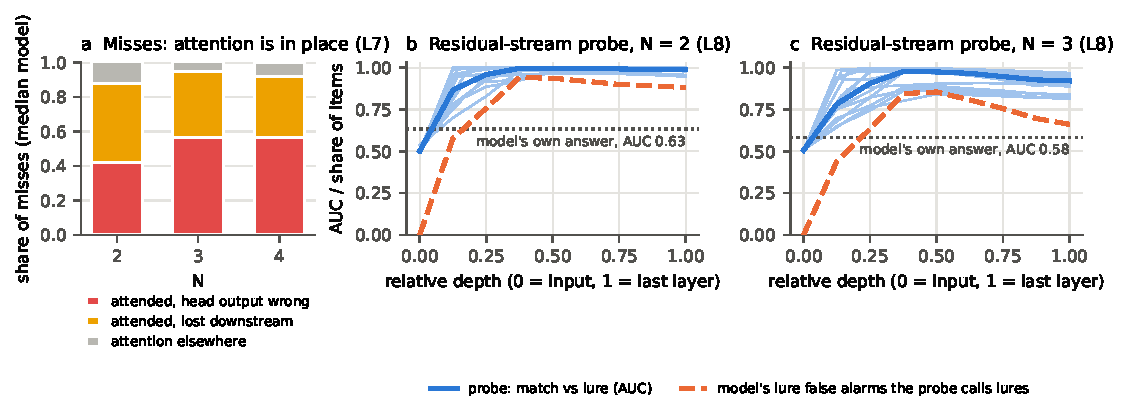
\includegraphics[width=\textwidth]{fig4_locate_vs_readout.pdf}
  \caption{\textbf{Locating versus readout.} (a) Misses split by whether the top heads attended to the target line and whether their output carried the right answer (median model). (b, c) A probe separates matches from lures by the position of the matching letter (blue; thin lines are models) and recognizes most of the model's own lure false alarms (orange), far above the model's own answer (dotted).}
  \label{fig:locate}
\end{figure}

\section{Causal tests: sharpening versus removing interference}
\label{sec:causal}

We apply five interventions to all 15 models at N = 2--4, on the same sequences, each with its own calibrated threshold (Fig.~\ref{fig:causal}; Table~\ref{tab:b1}). Intervals are 95\% paired bootstrap intervals over sequences (2,000 resamples); two degenerate cells whose baseline \dprime{} is below 0.3 are excluded.
\begin{itemize}
  \item \textbf{Ablation.} Mean-ablating the top-10 patching heads lowers \dprime{} in 42 of 43 cells (median $-0.93$); ten random heads from the same layers do not (median $+0.00$). The effect shrinks with scale (Qwen2.5-7B: $-0.27$ to $+0.03$; Qwen2.5-14B: $-0.48$ to $-0.17$), indicating more distributed solutions.
  \item \textbf{Sharpening.} Scaling the top-3 heads' logits by $1/\tau$ changes \dprime{} by a median $+0.05$ at $\tau=0.67$ and $+0.03$ at $\tau=0.8$ (range $-0.30$ to $+0.30$); flattening them ($\tau=2$) costs a median 0.32 in the full sweep. Changing the temperature of every head helps most at mild \emph{flattening} ($\tau=1.25$) in 19 of 30 cells. The heads sit near their optimal sharpness.
  \item \textbf{Distractor suppression.} For each query $i$, we remove the 19-dimensional letter-identity subspace (fit on calibration sequences at every residual site) from the whole line of every earlier item except $i-N$, scoring each query on its own prefix. At half strength this raises \dprime{} in 42 of 43 cells (median $+0.60$, up to $+1.78$), including at N = 4 (median $+0.44$) and in Qwen2.5-14B ($1.60\to3.38$ at N = 3). False alarms fall from about 0.2--0.3 to about 0.1 while hits hold. Removing a random subspace of the same rank does nothing (median $-0.03$); removing the target's letter destroys performance (median $-1.54$). Full strength also helps (median $+0.46$) but over-suppresses in Qwen2.5-7B.
  \item \textbf{Replication of \citet{xiong2026superposition}.} One letter-identity direction at one of the two earliest depths, applied at answer positions only, with the configuration chosen on calibration sequences: median $+0.11$ (range $+0.01$ to $+0.30$, 28 cells). The best-of-sweep statistic selected on test data gives $+0.12$, so their effect replicates; it is about a fifth of the effect of targeting the distractor items.
\end{itemize}
Across cells, distractor suppression and head ablation differ from zero with Wilcoxon $p<10^{-8}$; sharpening gives a small but consistent gain ($p=0.04$ at $\tau=0.67$, $p=0.001$ at $\tau=0.8$), an order of magnitude below distractor suppression. Distractor suppression is oracle-targeted, since it knows which item is the target, so it is a causal test of interference rather than a usable method.

\textbf{Scale.} The two accounts part ways as models grow (Fig.~\ref{fig:causal}b). Ablating the identified heads costs less in larger models (Spearman $\rho=0.74$ between size and each model's median change, $p=0.002$, 15 models), from about $-1.6$ in the smallest Pythia models to $-0.21$ in Qwen2.5-14B: the solution becomes more distributed. Removing distractor content helps more ($\rho=0.57$, $p=0.03$, 15 models). Qwen2.5-14B, the largest model, shows the pattern most clearly. Half-strength suppression raises its \dprime{} from 2.42 to 2.88, 1.60 to 3.38 and 1.29 to 2.05 at N = 2, 3 and 4, with every bootstrap interval at least 0.40 above zero; a random subspace of the same rank changes it by $-0.10$, $-0.05$ and $+0.18$. With distractor content removed, the model at N = 3 outperforms its own unmodified N = 2 baseline. Scale makes the task less dependent on a few heads, but not less limited by interference.

\begin{figure}[t]
  \centering
  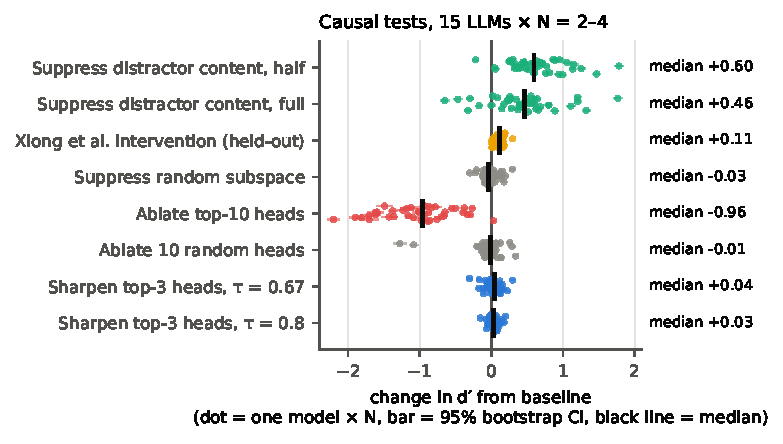
\includegraphics[width=\textwidth]{fig5_causal_tests.pdf}
  \caption{\textbf{Causal tests.} (a) Change in \dprime{} from baseline for each intervention; each dot is one model $\times$ N cell with its 95\% bootstrap interval, black lines are medians. (b) Each model's median change over N = 2--4 against its size, for distractor suppression (half strength) and top-10 head ablation; lines are least-squares fits in log size.}
  \label{fig:causal}
\end{figure}

\section{Architectures and development}
\label{sec:arch}

Recurrent baselines trained on the same stimuli separate two kinds of memory (Fig.~\ref{fig:arch}a,b). LSTM and LRU with a 512-dimensional state solve every N (\dprime{} $\ge7.9$); with a 32-dimensional state the LSTM declines (8.2 to 1.8) while the LRU barely does. Linear attention declines at both sizes, and a selective state-space model, whose gating is input-dependent like attention, declines from 8.2 to 2.9 even with a 512-dimensional state. The decline is not specific to softmax attention; it appears in architectures that retrieve by content-dependent weighting. In Pythia, the top N-back heads and the behaviour appear early in training: \dprime{} at N = 2 rises from chance to near its final value between steps 1,000 and 8,000, alongside previous-token and induction heads (Fig.~\ref{fig:arch}c).

\begin{figure}[t]
  \centering
  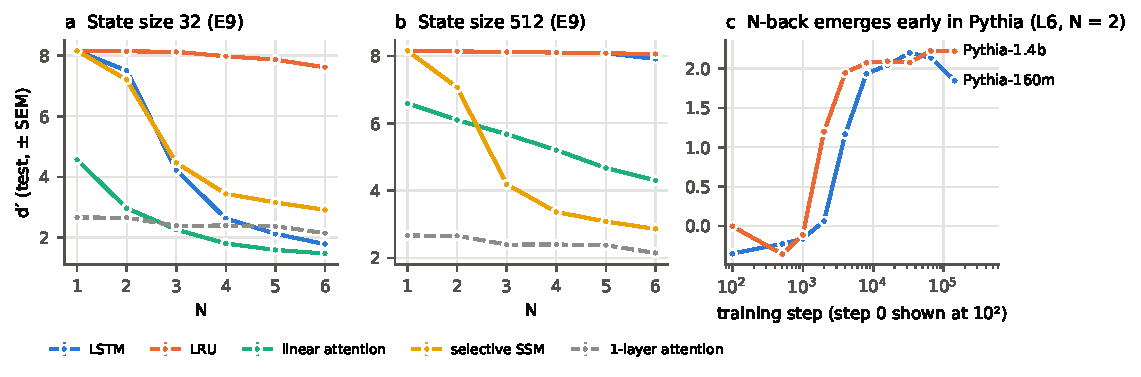
\includegraphics[width=\textwidth]{fig6_architectures_development.pdf}
  \caption{\textbf{Architectures and development.} (a, b) Recurrent and linear-attention baselines at state sizes 32 and 512, with the one-layer attention model (dashed) for reference; LSTM-512 overlaps LRU-512. (c) N-back \dprime{} over Pythia training (N = 2).}
  \label{fig:arch}
\end{figure}

\section{Discussion and limitations}
\label{sec:discussion}

Pretrained transformers locate the item N back: content-addressed heads land on the target line, and the residual stream encodes whether the matching letter sat at $i-N$ or at a lure position. They fail in readout, where the content of other items interferes with the decision. Sharpening attention cannot fix this; removing the interfering content largely does. The precision account is not wrong so much as narrow: it describes a one-layer, residual-free model, and depth removes it. This places transformer working memory closer to interference accounts of human working memory than to fixed-slot or attention-bottleneck accounts \citep{ma2014changing,engle2002executive}, and suggests that training or architectural changes that separate item content from the decision variable, rather than sharper attention, are the lever for improving it.

\textbf{Limitations.} We study one task family (letter N-back) with synthetic stimuli. The mechanistic analyses use the line format and the feedback condition. Models range up to 14B parameters, and the identified heads matter less in larger models, so the head-level account may not transfer to frontier models, although the suppression effect grows rather than shrinks with scale in our range (Fig.~\ref{fig:causal}b). Distractor suppression requires knowing the target and is a diagnostic, not a method. The probes show that information is linearly present, not that the model could use it with its existing weights. Our theory is limited to the minimal model.

\textbf{Broader impact.} This is basic research on model mechanisms with public models and synthetic data. Better diagnosis of working-memory failures may help evaluation; the interventions are analysis tools with no deployment use.

\bibliographystyle{plainnat}
\bibliography{refs}

\appendix

\section{Proofs}
\label{app:theory}

\textbf{Proposition~\ref{prop:mass}.} Let $e_x$ be the value vector of letter $x$ (no residual stream, no MLP, so the output is $o_i=\sum_j a_{ij}e_{x_j}$ up to a fixed linear map, plus positional components that do not depend on the letters). A linear readout computes $w^\top o_i=\sum_j a_{ij}w^\top e_{x_j}$. For fixed attention weights this is additive in the letters, so it cannot represent the indicator $[x_i=x_{i-N}]$, which is not additive (it is an XOR-like function of the two letters). Any dependence of the decision on equality must enter through $a_{ij}$, which depends on $x_i$ and $x_j$ jointly through the content term $c(x_i,x_j)$. \qed

\textbf{Proposition~\ref{prop:dispersion}.} With target logit $s_t$ and $K$ competitors $s_k\le s_t-\Delta$, $a_t=e^{s_t}/(e^{s_t}+\sum_k e^{s_k})\ge 1/(1+Ke^{-\Delta})$. Requiring $a_t\ge1-\epsilon$ gives $Ke^{-\Delta}\le\epsilon/(1-\epsilon)$, so $\Delta\ge\log(K/\epsilon)+\log(1-\epsilon)$. For a lure $\ell$ with $x_\ell=x_t$, $c(x_i,x_\ell)=c(x_i,x_t)$ and $a_\ell/a_t=\exp(p(i-\ell)-p(i-t))=e^{-\delta_P}$. \qed

\textbf{Proposition~\ref{prop:depth}} (sketch). With absolute positions $P_j$ and a first-layer head whose query--key product is $\beta\,P_i^\top R P_j$ with $R$ chosen so that $P_i^\top RP_j$ is maximized uniquely at $j=i-N$ with gap $g>0$, the head places mass at least $1/(1+Le^{-\beta g})$ on $i-N$; its output, added to the residual stream, makes $e_{x_{i-N}}$ available at position $i$ alongside $e_{x_i}$, and an MLP or a second attention layer can compute equality of the two letters. Rotary codes provide the same relative-offset selectivity. Under ALiBi, the bias $-m(i-j)$ is monotone in distance, so one head's maximum over positions with equal content is always the most recent, and offset $N>1$ cannot be singled out. \qed

\section{Methods}
\label{app:methods}

\textbf{Minimal models.} Attention-only transformers ($d_{\text{model}}=512$ for the main one-layer configuration, 128 for variants), Adam with learning rate $10^{-4}$, batch 32, fresh sequences each step, up to 30,000 steps with early stopping on validation loss (patience 2,000); 50 seeds for the main configuration (E1) and 10 for each variant. Variants: depth and residual stream, learned, sinusoidal, rotary, ALiBi and no position code, softmax, scalable softmax, sigmoid and top-$k$ attention; the cued multi-N model is a two-layer residual model with a cue token giving N. Recurrent baselines (LSTM, LRU, linear attention, selective SSM) use state sizes 32, 128 and 512.

\textbf{LLM evaluation.} Prompts start with a one-sentence instruction and ``N = $n$'', then three demonstration sequences with correct answers and the test sequence. Letters, ``\texttt{ m}'' and ``\texttt{ -}'' are single tokens in every tokenizer (checked per model). Models up to 1B run in float32 and larger models in bfloat16. The chat format sends one user turn per letter and one assistant turn per answer.

\textbf{Head ranking (L3).} Clean and corrupted prompts differ only in the letter at $i-N$, flipping the answer. For each head we patch its output from the clean run into the corrupted run at all positions and report the recovered fraction of the mean logit-difference gap (set to missing when the gap is below 0.1).

\textbf{Locate analysis (L7).} Attention from the query letter token to all tokens of a line is summed per head and averaged over the top-5 heads. The answer probe is a logistic regression on the top-5 heads' outputs at the query, trained on up to 4,000 correct items and applied to errors.

\textbf{Probe (L8).} Items with a same-letter item at $i-N$ (matches) or at a lure offset (lures); logistic regression with $L_2$ penalty on standardized features, five folds split by sequence.

\textbf{Interventions (L5, B1).} Sharpening multiplies a head's attention logits by $1/\tau$; ablation replaces a head's output by its mean over calibration items; random heads are drawn from the same layers. Suppression replaces $h$ by $h-\alpha\,((h-\mu)U)U^\top$ at every residual site (input to the first layer and every layer's output) over the tokens of each non-target line, where $U$ spans the 19 centred class means of the 20 letters at test-item letter tokens. The random control uses a random orthonormal $U$ of the same rank.

\textbf{Compute.} Minimal models mostly on a CPU cluster (about 1,060 core-hours), with some sweeps on single H100 GPUs; LLM studies on single L40S, H100 or B200 GPUs per model and N. The whole project, including preliminary and failed runs, used about \gpuhours{} GPU-hours.

\textbf{Licenses.} Pythia (Apache-2.0), GPT-2 (MIT), Qwen2.5 (Apache-2.0; Qwen license for some sizes).

\section{Additional results}
\label{app:results}

\begin{table}[h]
  \centering\small
  \caption{\dprime{} by model and N (line format, feedback condition), and false-alarm rates on N$\pm$1 lures versus non-lure items at N = 2.}
  \label{tab:l2}
  \begin{tabular}{lrrrrrrr}
\toprule
Model & $N{=}1$ & 2 & 3 & 4 & 5 & 6 & lure FA, $N{=}2$ \\
\midrule
Pythia-70m & 1.25 & 1.52 & 1.40 & 0.03 & 0.45 & -0.06 & 0.83 / 0.12 \\
Pythia-160m & 2.10 & 1.85 & 1.92 & 0.96 & 0.79 & 0.10 & 0.79 / 0.02 \\
Pythia-410m & 2.37 & 1.76 & 1.25 & 0.53 & 0.56 & 0.44 & 0.76 / 0.04 \\
Pythia-1b & 2.57 & 2.06 & 1.46 & 0.64 & 0.73 & 0.54 & 0.83 / 0.04 \\
Pythia-1.4b & 3.03 & 2.21 & 1.36 & 0.99 & 0.74 & 0.80 & 0.73 / 0.02 \\
Pythia-2.8b & 2.71 & 2.10 & 1.42 & 0.94 & 0.87 & 0.63 & 0.82 / 0.03 \\
Pythia-6.9b & 3.19 & 1.93 & 1.26 & 1.07 & 1.08 & 1.00 & 0.64 / 0.03 \\
GPT-2 & 2.15 & 2.08 & 1.28 & 0.87 & 0.73 & -0.02 & 0.96 / 0.08 \\
GPT-2 medium & 2.27 & 1.92 & 1.35 & 0.95 & 0.89 & 0.50 & 0.92 / 0.06 \\
GPT-2 large & 2.36 & 2.24 & 1.43 & 0.91 & 0.67 & 0.21 & 0.95 / 0.04 \\
GPT-2 xl & 2.34 & 1.48 & 0.93 & -0.01 & 0.16 & 0.15 & 0.70 / 0.06 \\
Qwen2.5-0.5B & 2.58 & 1.64 & 1.04 & 0.64 & 0.52 & 0.52 & 0.81 / 0.06 \\
Qwen2.5-1.5B & 2.86 & 2.18 & 1.75 & 1.18 & 1.26 & 0.76 & 0.65 / 0.01 \\
Qwen2.5-7B & 3.17 & 1.53 & 1.44 & 0.88 & 0.61 & 0.79 & 0.64 / 0.06 \\
Qwen2.5-14B & 4.28 & 2.42 & 1.60 & 1.29 & 1.41 & 1.15 & 0.63 / 0.01 \\
\bottomrule
\end{tabular}

\end{table}

\begin{table}[h]
  \centering\small
  \caption{Change in \dprime{} under each intervention; bold entries have 95\% bootstrap intervals excluding zero. $^\dagger$ degenerate baseline (excluded from summaries).}
  \label{tab:b1}
  \begin{tabular}{lrrrrrrr}
\toprule
Model & $N$ & base $d'$ & sharpen & ablate top & ablate rand. & suppress & supp. rand. \\
\midrule
Pythia-70m & 2 & 1.52 & \textbf{-0.11} & \textbf{-1.71} & \textbf{-1.08} & \textbf{+0.38} & \textbf{-0.30} \\
 & 3 & 1.40 & \textbf{+0.22} & \textbf{-1.49} & \textbf{-1.28} & \textbf{+0.05} & \textbf{-0.21} \\
 & 4 & 0.03$^\dagger$ & \textbf{+0.97} & \textbf{-0.17} & +0.04 & \textbf{+0.82} & \textbf{+0.31} \\
\addlinespace[2pt]
Pythia-160m & 2 & 1.85 & \textbf{+0.14} & \textbf{-1.62} & +0.01 & \textbf{+1.25} & \textbf{+0.29} \\
 & 3 & 1.92 & \textbf{-0.17} & \textbf{-1.90} & \textbf{-0.13} & \textbf{+0.30} & +0.03 \\
 & 4 & 0.96 & \textbf{+0.30} & \textbf{-1.09} & \textbf{-0.20} & \textbf{-0.22} & +0.01 \\
\addlinespace[2pt]
Pythia-410m & 2 & 1.76 & \textbf{+0.17} & \textbf{-1.36} & \textbf{-0.03} & \textbf{+0.61} & -0.01 \\
 & 3 & 1.25 & \textbf{-0.08} & \textbf{-1.18} & \textbf{+0.13} & \textbf{+0.60} & \textbf{-0.04} \\
 & 4 & 0.53 & \textbf{+0.13} & \textbf{-0.39} & \textbf{+0.08} & \textbf{+0.70} & \textbf{+0.05} \\
\addlinespace[2pt]
Pythia-1b & 2 & 2.06 & \textbf{-0.04} & \textbf{-1.81} & \textbf{+0.13} & \textbf{+0.59} & \textbf{-0.05} \\
 & 3 & 1.46 & \textbf{+0.11} & \textbf{-1.70} & \textbf{+0.34} & \textbf{+0.26} & \textbf{-0.12} \\
 & 4 & 0.64 & \textbf{+0.09} & \textbf{-0.83} & \textbf{+0.29} & \textbf{+0.39} & \textbf{-0.09} \\
\addlinespace[2pt]
Pythia-1.4b & 2 & 2.21 & \textbf{+0.08} & \textbf{-1.61} & \textbf{-0.06} & \textbf{+0.95} & \textbf{-0.05} \\
 & 3 & 1.36 & \textbf{+0.05} & \textbf{-0.93} & \textbf{+0.05} & \textbf{+0.46} & \textbf{+0.05} \\
 & 4 & 0.99 & \textbf{+0.05} & \textbf{-0.66} & +0.02 & \textbf{+0.44} & \textbf{-0.07} \\
\addlinespace[2pt]
Pythia-2.8b & 2 & 2.10 & \textbf{-0.05} & \textbf{-1.59} & \textbf{-0.12} & \textbf{+0.25} & \textbf{-0.03} \\
 & 3 & 1.42 & \textbf{+0.12} & \textbf{-1.01} & \textbf{-0.03} & \textbf{+0.34} & -0.01 \\
 & 4 & 0.94 & \textbf{+0.12} & \textbf{-0.70} & \textbf{+0.02} & \textbf{+0.41} & \textbf{+0.05} \\
\addlinespace[2pt]
Pythia-6.9b & 2 & 1.93 & \textbf{+0.03} & \textbf{-1.02} & \textbf{-0.08} & \textbf{+0.94} & \textbf{-0.08} \\
 & 3 & 1.26 & \textbf{+0.10} & \textbf{-0.34} & \textbf{+0.26} & \textbf{+1.47} & \textbf{+0.13} \\
 & 4 & 1.07 & \textbf{+0.07} & \textbf{-0.55} & +0.03 & \textbf{+1.13} & \textbf{+0.09} \\
\addlinespace[2pt]
GPT-2 & 2 & 2.08 & \textbf{-0.30} & \textbf{-2.20} & \textbf{-0.09} & \textbf{+0.05} & \textbf{-0.22} \\
 & 3 & 1.28 & -0.00 & \textbf{-1.12} & \textbf{-0.09} & \textbf{+0.71} & \textbf{-0.07} \\
 & 4 & 0.87 & \textbf{-0.02} & \textbf{-0.86} & \textbf{+0.07} & \textbf{+0.32} & \textbf{-0.12} \\
\addlinespace[2pt]
GPT-2 medium & 2 & 1.92 & +0.02 & \textbf{-1.38} & \textbf{+0.14} & \textbf{+1.05} & +0.00 \\
 & 3 & 1.35 & \textbf{-0.06} & \textbf{-1.43} & \textbf{-0.10} & \textbf{+0.86} & \textbf{-0.08} \\
 & 4 & 0.95 & \textbf{-0.07} & \textbf{-0.98} & \textbf{-0.18} & \textbf{+0.34} & \textbf{-0.12} \\
\addlinespace[2pt]
GPT-2 large & 2 & 2.24 & \textbf{-0.17} & \textbf{-1.16} & \textbf{-0.09} & \textbf{+0.68} & \textbf{+0.06} \\
 & 3 & 1.43 & \textbf{+0.15} & \textbf{-0.89} & \textbf{+0.02} & \textbf{+0.77} & \textbf{-0.03} \\
 & 4 & 0.91 & \textbf{+0.06} & \textbf{-0.50} & \textbf{-0.05} & \textbf{+0.55} & \textbf{-0.03} \\
\addlinespace[2pt]
GPT-2 xl & 2 & 1.46 & \textbf{+0.12} & \textbf{-1.24} & \textbf{-0.06} & \textbf{+0.52} & \textbf{+0.15} \\
 & 3 & 0.94 & \textbf{+0.12} & \textbf{-0.88} & +0.01 & \textbf{+0.81} & \textbf{-0.05} \\
 & 4 & -0.02$^\dagger$ & \textbf{+0.55} & \textbf{-0.16} & \textbf{+0.53} & \textbf{+0.91} & \textbf{+0.48} \\
\addlinespace[2pt]
Qwen2.5-0.5B & 2 & 1.64 & \textbf{-0.03} & \textbf{-0.87} & \textbf{+0.06} & \textbf{+0.49} & \textbf{+0.15} \\
 & 3 & 1.04 & \textbf{+0.05} & \textbf{-0.65} & \textbf{-0.11} & \textbf{+0.67} & \textbf{-0.07} \\
 & 4 & 0.64 & -0.01 & \textbf{-0.38} & +0.02 & \textbf{+0.60} & \textbf{-0.09} \\
\addlinespace[2pt]
Qwen2.5-1.5B & 2 & 2.18 & \textbf{+0.10} & \textbf{-0.76} & \textbf{+0.06} & \textbf{+0.89} & \textbf{-0.11} \\
 & 3 & 1.75 & +0.01 & \textbf{-0.93} & \textbf{-0.05} & \textbf{+1.15} & +0.01 \\
 & 4 & 1.18 & \textbf{-0.04} & \textbf{-0.78} & \textbf{-0.11} & \textbf{+0.28} & \textbf{-0.09} \\
\addlinespace[2pt]
Qwen2.5-7B & 2 & 1.53 & +0.01 & \textbf{-0.27} & \textbf{+0.06} & \textbf{+0.41} & \textbf{+0.04} \\
 & 3 & 1.44 & \textbf{-0.11} & \textbf{-0.29} & -0.02 & \textbf{+0.99} & \textbf{+0.20} \\
 & 4 & 0.88 & +0.00 & +0.03 & +0.00 & \textbf{+0.63} & \textbf{+0.14} \\
\addlinespace[2pt]
Qwen2.5-14B & 2 & 2.42 & \textbf{+0.05} & \textbf{-0.48} & \textbf{-0.04} & \textbf{+0.46} & \textbf{-0.10} \\
 & 3 & 1.60 & +0.01 & \textbf{-0.17} & +0.01 & \textbf{+1.78} & \textbf{-0.05} \\
 & 4 & 1.29 & \textbf{+0.13} & \textbf{-0.21} & \textbf{+0.07} & \textbf{+0.76} & \textbf{+0.18} \\
\addlinespace[2pt]
\bottomrule
\end{tabular}

\end{table}

\begin{table}[h]
  \centering\small
  \caption{Locate (L7) and probe (L8) results per model.}
  \label{tab:l7l8}
  \begin{tabular}{lrrrrrrr}
\toprule
& & \multicolumn{3}{c}{L7: share of misses} & \multicolumn{3}{c}{L8: match vs.\ lure} \\
\cmidrule(lr){3-5}\cmidrule(lr){6-8}
Model & $N$ & elsewhere & lost later & head wrong & model AUC & probe AUC & FA called lure \\
\midrule
Pythia-70m & 2 & 0.08 & 0.49 & 0.43 & 0.58 & 0.97 & 0.75 \\
 & 3 & 0.01 & 0.42 & 0.57 & 0.57 & 0.91 & 0.61 \\
Pythia-160m & 2 & 0.26 & 0.34 & 0.40 & 0.63 & 0.98 & 0.82 \\
 & 3 & 0.03 & 0.59 & 0.38 & 0.58 & 0.99 & 0.85 \\
Pythia-410m & 2 & 0.11 & 0.36 & 0.53 & 0.66 & 1.00 & 0.95 \\
 & 3 & 0.06 & 0.40 & 0.54 & 0.58 & 0.98 & 0.84 \\
Pythia-1b & 2 & 0.11 & 0.32 & 0.57 & 0.68 & 1.00 & 0.95 \\
 & 3 & 0.06 & 0.30 & 0.64 & 0.60 & 0.98 & 0.87 \\
Pythia-1.4b & 2 & 0.12 & 0.72 & 0.16 & 0.76 & 1.00 & 0.99 \\
 & 3 & 0.06 & 0.38 & 0.56 & 0.62 & 0.99 & 0.92 \\
Pythia-2.8b & 2 & 0.04 & 0.36 & 0.60 & 0.71 & 1.00 & 1.00 \\
 & 3 & 0.04 & 0.38 & 0.58 & 0.60 & 1.00 & 0.96 \\
Pythia-6.9b & 2 & 0.19 & 0.55 & 0.26 & 0.74 & 1.00 & 1.00 \\
 & 3 & 0.08 & 0.38 & 0.54 & 0.60 & 1.00 & 0.98 \\
GPT-2 & 2 & 0.16 & 0.65 & 0.19 & 0.49 & 0.97 & 0.84 \\
 & 3 & 0.12 & 0.38 & 0.50 & 0.48 & 0.84 & 0.53 \\
GPT-2 medium & 2 & 0.18 & 0.53 & 0.29 & 0.48 & 0.99 & 0.87 \\
 & 3 & 0.07 & 0.39 & 0.54 & 0.47 & 0.86 & 0.57 \\
GPT-2 large & 2 & 0.72 & 0.15 & 0.13 & 0.56 & 0.99 & 0.92 \\
 & 3 & 0.54 & 0.20 & 0.26 & 0.50 & 0.88 & 0.59 \\
GPT-2 xl & 2 & 0.15 & 0.42 & 0.43 & 0.60 & 1.00 & 0.92 \\
 & 3 & 0.10 & 0.28 & 0.62 & 0.49 & 0.89 & 0.69 \\
Qwen2.5-0.5B & 2 & 0.16 & 0.50 & 0.34 & 0.62 & 1.00 & 1.00 \\
 & 3 & 0.09 & 0.23 & 0.67 & 0.53 & 0.99 & 0.91 \\
Qwen2.5-1.5B & 2 & 0.17 & 0.42 & 0.41 & 0.78 & 1.00 & 1.00 \\
 & 3 & 0.04 & 0.39 & 0.57 & 0.67 & 0.99 & 0.86 \\
Qwen2.5-7B & 2 & 0.14 & 0.43 & 0.43 & 0.63 & 1.00 & 0.98 \\
 & 3 & 0.45 & 0.19 & 0.36 & 0.60 & 0.98 & 0.88 \\
Qwen2.5-14B & 2 & 0.68 & 0.17 & 0.14 & 0.81 & 1.00 & 1.00 \\
 & 3 & 0.51 & 0.13 & 0.36 & 0.64 & 1.00 & 0.95 \\
\bottomrule
\end{tabular}

\end{table}

\textbf{Post-hoc attention edits in the minimal model (E7).} On 720 one-layer checkpoints, a fixed split of attention between $i$ and $i-N$ gives \dprime{}~$\approx0$ at every N; keeping only the model's own mass on $i$ and $i-N$ lowers \dprime{} from 2.70 to 0.63 at N = 1 and from 2.18 to 1.32 at N = 6, with false alarms rising from 0.03 to 0.67 at N = 1. Removing either the content or the position term of the logits gives \dprime{}~$\approx0$.

\clearpage
\section*{NeurIPS Paper Checklist}




\begin{enumerate}

\item {\bf Claims}
    \item[] Question: Do the main claims made in the abstract and introduction accurately reflect the paper's contributions and scope?
    \item[] Answer: \answerYes{} % Replace by \answerYes{}, \answerNo{}, or \answerNA{}.
    \item[] Justification: The abstract and Section~\ref{sec:intro} state the four claims (decomposition, causal contrast, where precision binds, architectures); each maps to Sections~\ref{sec:theory}--\ref{sec:causal} and states its scope (15 base models up to 14B parameters, letter N-back).
    \item[] Guidelines:
    \begin{itemize}
        \item The answer \answerNA{} means that the abstract and introduction do not include the claims made in the paper.
        \item The abstract and/or introduction should clearly state the claims made, including the contributions made in the paper and important assumptions and limitations. A \answerNo{} or \answerNA{} answer to this question will not be perceived well by the reviewers. 
        \item The claims made should match theoretical and experimental results, and reflect how much the results can be expected to generalize to other settings. 
        \item It is fine to include aspirational goals as motivation as long as it is clear that these goals are not attained by the paper. 
    \end{itemize}

\item {\bf Limitations}
    \item[] Question: Does the paper discuss the limitations of the work performed by the authors?
    \item[] Answer: \answerYes{} % Replace by \answerYes{}, \answerNo{}, or \answerNA{}.
    \item[] Justification: Section~\ref{sec:discussion} lists the limitations: one task family, oracle-targeted suppression, models up to 14B, and line-format prompts for the mechanistic studies.
    \item[] Guidelines:
    \begin{itemize}
        \item The answer \answerNA{} means that the paper has no limitation while the answer \answerNo{} means that the paper has limitations, but those are not discussed in the paper. 
        \item The authors are encouraged to create a separate ``Limitations'' section in their paper.
        \item The paper should point out any strong assumptions and how robust the results are to violations of these assumptions (e.g., independence assumptions, noiseless settings, model well-specification, asymptotic approximations only holding locally). The authors should reflect on how these assumptions might be violated in practice and what the implications would be.
        \item The authors should reflect on the scope of the claims made, e.g., if the approach was only tested on a few datasets or with a few runs. In general, empirical results often depend on implicit assumptions, which should be articulated.
        \item The authors should reflect on the factors that influence the performance of the approach. For example, a facial recognition algorithm may perform poorly when image resolution is low or images are taken in low lighting. Or a speech-to-text system might not be used reliably to provide closed captions for online lectures because it fails to handle technical jargon.
        \item The authors should discuss the computational efficiency of the proposed algorithms and how they scale with dataset size.
        \item If applicable, the authors should discuss possible limitations of their approach to address problems of privacy and fairness.
        \item While the authors might fear that complete honesty about limitations might be used by reviewers as grounds for rejection, a worse outcome might be that reviewers discover limitations that aren't acknowledged in the paper. The authors should use their best judgment and recognize that individual actions in favor of transparency play an important role in developing norms that preserve the integrity of the community. Reviewers will be specifically instructed to not penalize honesty concerning limitations.
    \end{itemize}

\item {\bf Theory assumptions and proofs}
    \item[] Question: For each theoretical result, does the paper provide the full set of assumptions and a complete (and correct) proof?
    \item[] Answer: \answerYes{} % Replace by \answerYes{}, \answerNo{}, or \answerNA{}.
    \item[] Justification: The propositions and corollaries in Section~\ref{sec:theory} state their assumptions (Propositions 1--3: one layer, no residual stream, no MLP, alphabet-symmetric stimuli; Proposition~\ref{prop:interference}: a linear readout with additive distractor content); proofs are in Appendix~\ref{app:theory}, and Proposition~\ref{prop:depth} is given as a constructive sketch.
    \item[] Guidelines:
    \begin{itemize}
        \item The answer \answerNA{} means that the paper does not include theoretical results. 
        \item All the theorems, formulas, and proofs in the paper should be numbered and cross-referenced.
        \item All assumptions should be clearly stated or referenced in the statement of any theorems.
        \item The proofs can either appear in the main paper or the supplemental material, but if they appear in the supplemental material, the authors are encouraged to provide a short proof sketch to provide intuition. 
        \item Inversely, any informal proof provided in the core of the paper should be complemented by formal proofs provided in appendix or supplemental material.
        \item Theorems and Lemmas that the proof relies upon should be properly referenced. 
    \end{itemize}

    \item {\bf Experimental result reproducibility}
    \item[] Question: Does the paper fully disclose all the information needed to reproduce the main experimental results of the paper to the extent that it affects the main claims and/or conclusions of the paper (regardless of whether the code and data are provided or not)?
    \item[] Answer: \answerYes{} % Replace by \answerYes{}, \answerNo{}, or \answerNA{}.
    \item[] Justification: Section~\ref{sec:setup} and Appendix~\ref{app:methods} give stimuli, prompts, thresholds, model lists, head selection, intervention definitions and all hyperparameters.
    \item[] Guidelines:
    \begin{itemize}
        \item The answer \answerNA{} means that the paper does not include experiments.
        \item If the paper includes experiments, a \answerNo{} answer to this question will not be perceived well by the reviewers: Making the paper reproducible is important, regardless of whether the code and data are provided or not.
        \item If the contribution is a dataset and\slash or model, the authors should describe the steps taken to make their results reproducible or verifiable. 
        \item Depending on the contribution, reproducibility can be accomplished in various ways. For example, if the contribution is a novel architecture, describing the architecture fully might suffice, or if the contribution is a specific model and empirical evaluation, it may be necessary to either make it possible for others to replicate the model with the same dataset, or provide access to the model. In general. releasing code and data is often one good way to accomplish this, but reproducibility can also be provided via detailed instructions for how to replicate the results, access to a hosted model (e.g., in the case of a large language model), releasing of a model checkpoint, or other means that are appropriate to the research performed.
        \item While NeurIPS does not require releasing code, the conference does require all submissions to provide some reasonable avenue for reproducibility, which may depend on the nature of the contribution. For example
        \begin{enumerate}
            \item If the contribution is primarily a new algorithm, the paper should make it clear how to reproduce that algorithm.
            \item If the contribution is primarily a new model architecture, the paper should describe the architecture clearly and fully.
            \item If the contribution is a new model (e.g., a large language model), then there should either be a way to access this model for reproducing the results or a way to reproduce the model (e.g., with an open-source dataset or instructions for how to construct the dataset).
            \item We recognize that reproducibility may be tricky in some cases, in which case authors are welcome to describe the particular way they provide for reproducibility. In the case of closed-source models, it may be that access to the model is limited in some way (e.g., to registered users), but it should be possible for other researchers to have some path to reproducing or verifying the results.
        \end{enumerate}
    \end{itemize}


\item {\bf Open access to data and code}
    \item[] Question: Does the paper provide open access to the data and code, with sufficient instructions to faithfully reproduce the main experimental results, as described in supplemental material?
    \item[] Answer: \answerYes{} % Replace by \answerYes{}, \answerNo{}, or \answerNA{}.
    \item[] Justification: Code, configs, stimuli generators and per-sequence scores will be released (anonymized repository in the supplement); all models are public checkpoints.
    \item[] Guidelines:
    \begin{itemize}
        \item The answer \answerNA{} means that paper does not include experiments requiring code.
        \item Please see the NeurIPS code and data submission guidelines (\url{https://neurips.cc/public/guides/CodeSubmissionPolicy}) for more details.
        \item While we encourage the release of code and data, we understand that this might not be possible, so \answerNo{} is an acceptable answer. Papers cannot be rejected simply for not including code, unless this is central to the contribution (e.g., for a new open-source benchmark).
        \item The instructions should contain the exact command and environment needed to run to reproduce the results. See the NeurIPS code and data submission guidelines (\url{https://neurips.cc/public/guides/CodeSubmissionPolicy}) for more details.
        \item The authors should provide instructions on data access and preparation, including how to access the raw data, preprocessed data, intermediate data, and generated data, etc.
        \item The authors should provide scripts to reproduce all experimental results for the new proposed method and baselines. If only a subset of experiments are reproducible, they should state which ones are omitted from the script and why.
        \item At submission time, to preserve anonymity, the authors should release anonymized versions (if applicable).
        \item Providing as much information as possible in supplemental material (appended to the paper) is recommended, but including URLs to data and code is permitted.
    \end{itemize}


\item {\bf Experimental setting/details}
    \item[] Question: Does the paper specify all the training and test details (e.g., data splits, hyperparameters, how they were chosen, type of optimizer) necessary to understand the results?
    \item[] Answer: \answerYes{} % Replace by \answerYes{}, \answerNo{}, or \answerNA{}.
    \item[] Justification: Appendix~\ref{app:methods} lists training settings for the minimal models (optimizer, learning rate, steps, early stopping, seeds) and evaluation settings for the LLMs.
    \item[] Guidelines:
    \begin{itemize}
        \item The answer \answerNA{} means that the paper does not include experiments.
        \item The experimental setting should be presented in the core of the paper to a level of detail that is necessary to appreciate the results and make sense of them.
        \item The full details can be provided either with the code, in appendix, or as supplemental material.
    \end{itemize}

\item {\bf Experiment statistical significance}
    \item[] Question: Does the paper report error bars suitably and correctly defined or other appropriate information about the statistical significance of the experiments?
    \item[] Answer: \answerYes{} % Replace by \answerYes{}, \answerNo{}, or \answerNA{}.
    \item[] Justification: Minimal-model results report mean $\pm$ SEM over 10--50 seeds; LLM interventions report 95\% paired sequence-level bootstrap intervals (2,000 resamples) and Wilcoxon tests across model $\times$ N cells (Section~\ref{sec:causal}).
    \item[] Guidelines:
    \begin{itemize}
        \item The answer \answerNA{} means that the paper does not include experiments.
        \item The authors should answer \answerYes{} if the results are accompanied by error bars, confidence intervals, or statistical significance tests, at least for the experiments that support the main claims of the paper.
        \item The factors of variability that the error bars are capturing should be clearly stated (for example, train/test split, initialization, random drawing of some parameter, or overall run with given experimental conditions).
        \item The method for calculating the error bars should be explained (closed form formula, call to a library function, bootstrap, etc.)
        \item The assumptions made should be given (e.g., Normally distributed errors).
        \item It should be clear whether the error bar is the standard deviation or the standard error of the mean.
        \item It is OK to report 1-sigma error bars, but one should state it. The authors should preferably report a 2-sigma error bar than state that they have a 96\% CI, if the hypothesis of Normality of errors is not verified.
        \item For asymmetric distributions, the authors should be careful not to show in tables or figures symmetric error bars that would yield results that are out of range (e.g., negative error rates).
        \item If error bars are reported in tables or plots, the authors should explain in the text how they were calculated and reference the corresponding figures or tables in the text.
    \end{itemize}

\item {\bf Experiments compute resources}
    \item[] Question: For each experiment, does the paper provide sufficient information on the computer resources (type of compute workers, memory, time of execution) needed to reproduce the experiments?
    \item[] Answer: \answerYes{} % Replace by \answerYes{}, \answerNo{}, or \answerNA{}.
    \item[] Justification: Appendix~\ref{app:methods} reports compute: mostly a CPU cluster for minimal models; single L40S, H100 or B200 GPUs per model and N for LLM studies; about \gpuhours{} GPU-hours in total, including preliminary and failed runs.
    \item[] Guidelines:
    \begin{itemize}
        \item The answer \answerNA{} means that the paper does not include experiments.
        \item The paper should indicate the type of compute workers CPU or GPU, internal cluster, or cloud provider, including relevant memory and storage.
        \item The paper should provide the amount of compute required for each of the individual experimental runs as well as estimate the total compute. 
        \item The paper should disclose whether the full research project required more compute than the experiments reported in the paper (e.g., preliminary or failed experiments that didn't make it into the paper). 
    \end{itemize}
    
\item {\bf Code of ethics}
    \item[] Question: Does the research conducted in the paper conform, in every respect, with the NeurIPS Code of Ethics \url{https://neurips.cc/public/EthicsGuidelines}?
    \item[] Answer: \answerYes{} % Replace by \answerYes{}, \answerNo{}, or \answerNA{}.
    \item[] Justification: The work uses public models and synthetic letter sequences, involves no human subjects or personal data, and conforms to the Code of Ethics.
    \item[] Guidelines:
    \begin{itemize}
        \item The answer \answerNA{} means that the authors have not reviewed the NeurIPS Code of Ethics.
        \item If the authors answer \answerNo, they should explain the special circumstances that require a deviation from the Code of Ethics.
        \item The authors should make sure to preserve anonymity (e.g., if there is a special consideration due to laws or regulations in their jurisdiction).
    \end{itemize}


\item {\bf Broader impacts}
    \item[] Question: Does the paper discuss both potential positive societal impacts and negative societal impacts of the work performed?
    \item[] Answer: \answerYes{} % Replace by \answerYes{}, \answerNo{}, or \answerNA{}.
    \item[] Justification: Section~\ref{sec:discussion} notes that the work is basic science on model mechanisms; better working-memory diagnosis could aid evaluation, and the interventions are analysis tools, not deployable capabilities.
    \item[] Guidelines:
    \begin{itemize}
        \item The answer \answerNA{} means that there is no societal impact of the work performed.
        \item If the authors answer \answerNA{} or \answerNo, they should explain why their work has no societal impact or why the paper does not address societal impact.
        \item Examples of negative societal impacts include potential malicious or unintended uses (e.g., disinformation, generating fake profiles, surveillance), fairness considerations (e.g., deployment of technologies that could make decisions that unfairly impact specific groups), privacy considerations, and security considerations.
        \item The conference expects that many papers will be foundational research and not tied to particular applications, let alone deployments. However, if there is a direct path to any negative applications, the authors should point it out. For example, it is legitimate to point out that an improvement in the quality of generative models could be used to generate Deepfakes for disinformation. On the other hand, it is not needed to point out that a generic algorithm for optimizing neural networks could enable people to train models that generate Deepfakes faster.
        \item The authors should consider possible harms that could arise when the technology is being used as intended and functioning correctly, harms that could arise when the technology is being used as intended but gives incorrect results, and harms following from (intentional or unintentional) misuse of the technology.
        \item If there are negative societal impacts, the authors could also discuss possible mitigation strategies (e.g., gated release of models, providing defenses in addition to attacks, mechanisms for monitoring misuse, mechanisms to monitor how a system learns from feedback over time, improving the efficiency and accessibility of ML).
    \end{itemize}
    
\item {\bf Safeguards}
    \item[] Question: Does the paper describe safeguards that have been put in place for responsible release of data or models that have a high risk for misuse (e.g., pre-trained language models, image generators, or scraped datasets)?
    \item[] Answer: \answerNA{} % Replace by \answerYes{}, \answerNo{}, or \answerNA{}.
    \item[] Justification: No high-risk models or datasets are released.
    \item[] Guidelines:
    \begin{itemize}
        \item The answer \answerNA{} means that the paper poses no such risks.
        \item Released models that have a high risk for misuse or dual-use should be released with necessary safeguards to allow for controlled use of the model, for example by requiring that users adhere to usage guidelines or restrictions to access the model or implementing safety filters. 
        \item Datasets that have been scraped from the Internet could pose safety risks. The authors should describe how they avoided releasing unsafe images.
        \item We recognize that providing effective safeguards is challenging, and many papers do not require this, but we encourage authors to take this into account and make a best faith effort.
    \end{itemize}

\item {\bf Licenses for existing assets}
    \item[] Question: Are the creators or original owners of assets (e.g., code, data, models), used in the paper, properly credited and are the license and terms of use explicitly mentioned and properly respected?
    \item[] Answer: \answerYes{} % Replace by \answerYes{}, \answerNo{}, or \answerNA{}.
    \item[] Justification: Pythia (Apache-2.0), GPT-2 (MIT), and Qwen2.5 (Apache-2.0 / Qwen license) are cited and used under their licenses (Appendix~\ref{app:methods}).
    \item[] Guidelines:
    \begin{itemize}
        \item The answer \answerNA{} means that the paper does not use existing assets.
        \item The authors should cite the original paper that produced the code package or dataset.
        \item The authors should state which version of the asset is used and, if possible, include a URL.
        \item The name of the license (e.g., CC-BY 4.0) should be included for each asset.
        \item For scraped data from a particular source (e.g., website), the copyright and terms of service of that source should be provided.
        \item If assets are released, the license, copyright information, and terms of use in the package should be provided. For popular datasets, \url{paperswithcode.com/datasets} has curated licenses for some datasets. Their licensing guide can help determine the license of a dataset.
        \item For existing datasets that are re-packaged, both the original license and the license of the derived asset (if it has changed) should be provided.
        \item If this information is not available online, the authors are encouraged to reach out to the asset's creators.
    \end{itemize}

\item {\bf New assets}
    \item[] Question: Are new assets introduced in the paper well documented and is the documentation provided alongside the assets?
    \item[] Answer: \answerYes{} % Replace by \answerYes{}, \answerNo{}, or \answerNA{}.
    \item[] Justification: The released code and stimulus generator are documented in the repository README.
    \item[] Guidelines:
    \begin{itemize}
        \item The answer \answerNA{} means that the paper does not release new assets.
        \item Researchers should communicate the details of the dataset\slash code\slash model as part of their submissions via structured templates. This includes details about training, license, limitations, etc. 
        \item The paper should discuss whether and how consent was obtained from people whose asset is used.
        \item At submission time, remember to anonymize your assets (if applicable). You can either create an anonymized URL or include an anonymized zip file.
    \end{itemize}

\item {\bf Crowdsourcing and research with human subjects}
    \item[] Question: For crowdsourcing experiments and research with human subjects, does the paper include the full text of instructions given to participants and screenshots, if applicable, as well as details about compensation (if any)? 
    \item[] Answer: \answerNA{} % Replace by \answerYes{}, \answerNo{}, or \answerNA{}.
    \item[] Justification: No crowdsourcing or human subjects.
    \item[] Guidelines:
    \begin{itemize}
        \item The answer \answerNA{} means that the paper does not involve crowdsourcing nor research with human subjects.
        \item Including this information in the supplemental material is fine, but if the main contribution of the paper involves human subjects, then as much detail as possible should be included in the main paper. 
        \item According to the NeurIPS Code of Ethics, workers involved in data collection, curation, or other labor should be paid at least the minimum wage in the country of the data collector. 
    \end{itemize}

\item {\bf Institutional review board (IRB) approvals or equivalent for research with human subjects}
    \item[] Question: Does the paper describe potential risks incurred by study participants, whether such risks were disclosed to the subjects, and whether Institutional Review Board (IRB) approvals (or an equivalent approval/review based on the requirements of your country or institution) were obtained?
    \item[] Answer: \answerNA{} % Replace by \answerYes{}, \answerNo{}, or \answerNA{}.
    \item[] Justification: No human subjects.
    \item[] Guidelines:
    \begin{itemize}
        \item The answer \answerNA{} means that the paper does not involve crowdsourcing nor research with human subjects.
        \item Depending on the country in which research is conducted, IRB approval (or equivalent) may be required for any human subjects research. If you obtained IRB approval, you should clearly state this in the paper. 
        \item We recognize that the procedures for this may vary significantly between institutions and locations, and we expect authors to adhere to the NeurIPS Code of Ethics and the guidelines for their institution. 
        \item For initial submissions, do not include any information that would break anonymity (if applicable), such as the institution conducting the review.
    \end{itemize}

\item {\bf Declaration of LLM usage}
    \item[] Question: Does the paper describe the usage of LLMs if it is an important, original, or non-standard component of the core methods in this research? Note that if the LLM is used only for writing, editing, or formatting purposes and does \emph{not} impact the core methodology, scientific rigor, or originality of the research, declaration is not required.
    %this research? 
    \item[] Answer: \answerYes{} % Replace by \answerYes{}, \answerNo{}, or \answerNA{}.
    \item[] Justification: Pretrained LLMs are the object of study. An AI coding assistant was also used to write analysis code, run experiments and draft text; all results were checked against the logged outputs by the authors.
    \item[] Guidelines:
    \begin{itemize}
        \item The answer \answerNA{} means that the core method development in this research does not involve LLMs as any important, original, or non-standard components.
        \item Please refer to our LLM policy in the NeurIPS handbook for what should or should not be described.
    \end{itemize}

\end{enumerate}

\end{document}
